% LaTeX Studio 演示样例：覆盖讲义生产的高频元素
% （目录两遍编译、行内/行间公式、矩阵、表格、中文、相对路径图片）。
% 模板头与 Java 生产链路 TeachingHandoutPdfExportService 保持一致（ctexart + geometry 2.4cm）。
\documentclass[UTF8]{ctexart}
\usepackage[margin=2.4cm]{geometry}
\usepackage{amsmath}
\usepackage{graphicx}
\usepackage{xcolor}

\definecolor{mainblue}{HTML}{4D6BFE}

\begin{document}
\begin{center}
  {\LARGE\bfseries 二次函数顶点式专题讲解}\\[4pt]
  {\small\color{gray} 高一 · 函数专题 · 教师版示例}
\end{center}

\tableofcontents

\section{知识速记}

二次函数的三种形式中，顶点式最能直接暴露图像的几何特征：
\begin{itemize}
  \item 顶点坐标：$\left(h,\ k\right)$，对称轴 $x=h$；
  \item 开口方向与宽窄：$a>0$ 开口向上，$|a|$ 越大开口越窄；
  \item 与一般式的关系：$y=ax^2+bx+c \iff h=-\dfrac{b}{2a},\ k=\dfrac{4ac-b^2}{4a}$。
\end{itemize}

\section{配方推导}

从一般式出发，通过配方法得到顶点式：
\begin{align*}
  y &= ax^2+bx+c \\
    &= a\left(x^2+\frac{b}{a}x\right)+c \\
    &= a\left(x+\frac{b}{2a}\right)^2 + c - a\cdot\frac{b^2}{4a^2} \\
    &= a\left(x+\frac{b}{2a}\right)^2 + \frac{4ac-b^2}{4a}.
\end{align*}

当 $a=2,\ b=-4,\ c=1$ 时：
\begin{equation}
  y = 2(x-1)^2 - 1,
\end{equation}
即顶点为 $(1,\,-1)$，最小值为 $-1$。

\section{图像平移族}

平移法则：左加右减（对 $x$）、上加下减（对整体）。

\begin{center}
  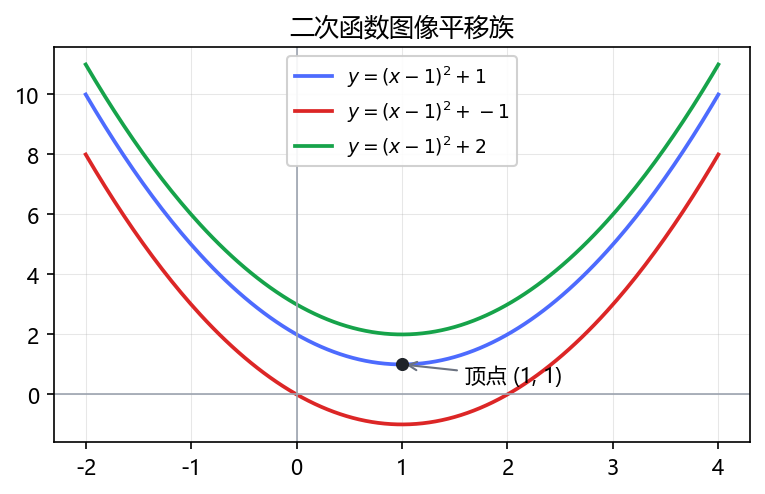
\includegraphics[width=0.72\textwidth]{figures/parabola.png}
\end{center}

\section{典型例题}

\subsection{例 1：求顶点与最值}

已知 $f(x)=3x^2-6x+5$，求其在区间 $[0,3]$ 上的最小值。

\begin{center}
\begin{tabular}{|c|c|c|}
  \hline
  \textbf{步骤} & \textbf{操作} & \textbf{结果} \\
  \hline
  配方 & $f(x)=3(x-1)^2+2$ & 顶点 $(1,2)$ \\
  \hline
  对称轴 & $x=1 \in [0,3]$ & 在区间内 \\
  \hline
  最小值 & $f(1)$ & $2$ \\
  \hline
\end{tabular}
\end{center}

\subsection{例 2：含参讨论}

设 $f(x)=x^2-2ax+3$ 在 $[1,3]$ 上的最小值为 $g(a)$，用矩阵形式记录分类：
\[
  \begin{pmatrix}
    a<1 & g(a)=4-2a \\
    1\le a\le 3 & g(a)=3-a^2 \\
    a>3 & g(a)=6-6a+3
  \end{pmatrix}
\]

\section{易错警示}

\begin{itemize}
  \item 顶点式 $y=a(x-h)^2+k$ 中的 $h$ 带符号：$y=2(x+1)^2-1$ 的顶点是 $(-1,-1)$ 而不是 $(1,-1)$；
  \item 区间最值要同时比较端点与顶点，不要默认顶点一定在区间内；
  \item \textcolor{red}{平移方向}：$y=(x-1)^2$ 是向\textbf{右}平移 $1$ 个单位。
\end{itemize}

\end{document}
